%\section{Vesicle traffic system background}
The phenomenology of vesicle traffic is unlikely to be familiar to many readers; however, the details are important for the rest of our discussion. 
%
Therefore, we give an overview of the molecular mechanism of the VTS and then we sketch out a few interesting problems that are key to an understanding of the VTS.
%
%\vspace{-0.5cm}
\subsection{Vesicle traffic system}
%Vesicles were discovered decades ago, in the early 1950s, and s
\noindent The major molecules involved in the VTS~\cite{wells2005discovery} can roughly be categorized as budding molecules, whose role is in the formation and budding of transport vesicles from the source compartment, and fusion molecules, which enable fusion of transport vesicles with the target compartments. 
%
Below, we give a brief description of the sequence of steps involved in the vesicle transport process. 
%
Through this description, we wish to provide a glimpse of the kind of molecular regulatory interactions that we encode in our model.
 
\begin{figure}
  \begin{center}
	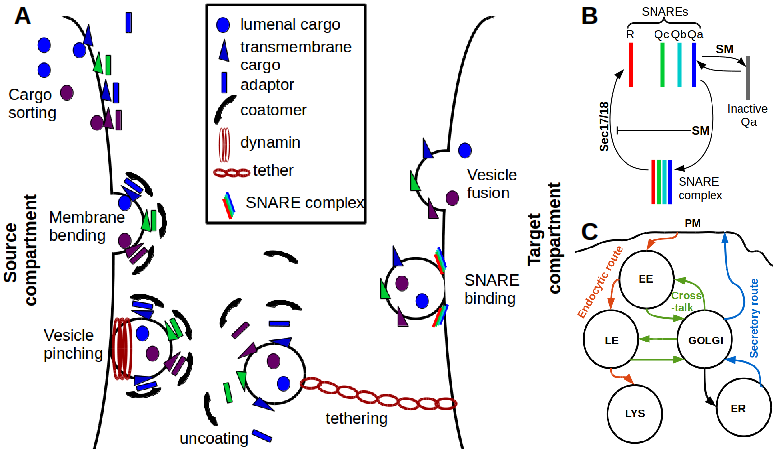
\includegraphics[height=9cm,width=12cm]{fig.png}
	\end{center}

	\caption{(A) Schematic of the vesicle transport system. Steps involved in vesicle transport between
		two compartments: a source and a target compartment, are shown. The symbols used for different
		molecules involved in vesicle traffic are explained in the key. At the source compartment,
		transmembrane cargo proteins are sorted by cytosolic adaptor proteins. Here, different colours
		indicate different types of cargo and adaptor proteins. Coat proteins are recruited to the forming
		vesicle by adaptor proteins. Note here that a single type of coat protein can interact with multiple
		types of adaptor proteins. Subsequently, the vesicle is pinched off at its neck, for example by dynamin
		protein. Once the vesicle has left the source compartment, the coat and adaptor proteins fall off and
		the vesicle is recognized and bound by a tethering complex which is linked to the target compartment.
		At the target compartment, the tethered vesicle undergoes fusion, thereby releasing its contents. (B)
		SNARE regulation network. Here, the dark blue, light blue, green and red stripes represent Qa, Qb,
		Qc and R SNAREs respectively. These 4 SNAREs interact to form a SNARE complex. SNARE
		complex formation is regulated by SM proteins and Sec 17/18. SM proteins inhibit SNARE complex
		formation by inactivating Qa SNAREs. They also enhance SNARE complex formation by stabilizing
		intermediate structures, and by inhibiting premature SNARE complex resolution. Sec17/18 aid in
		SNARE complex resolution. (C) A schematic of the typical eukaryotic cell's VTS. Large circles
		represent compartments, and edges represent vesicle routes. Identities of compartments are written
		inside or beside them; ER = endoplasmic reticulum, Golgi = Golgi apparatus, PM = plasma
		membrane, EE = early endosome, LE = late endosome, Lys = lysosome. The two major vesicle routes;
		the secretory and the endocytic routes are in blue and orange, respectively. The routes in green
		represent vesicles that allow cross-talk between the secretory and the endocytic routes. }
    \label{fig:vts}
\end{figure}

\subsubsection{Vesicle budding} 
The process of vesicle budding involves sorting and packaging of cargo molecules, membrane deformation and budding of the vesicle from the source compartment (Fig.~\ref{fig:vts}). 
%
Cargo sorting is performed by cytosolic adaptor proteins. 
%
Adaptor proteins bind to cargo molecules on the source
compartment and thereby sequester them for packaging \cite{paczkowski2015cargo}. 
%
Membrane deformation is caused by coat proteins which are recruited by adaptor proteins \cite{faini2013vesicle}. 
%
Although here we mention only these two molecule types, many other molecules play a role in regulation and orchestration of these processes.
%Next, cytosolic coat proteins are recruited to the forming vesicle through their interaction with adaptor proteins \cite{faini2013vesicle}. 
%
%Coat proteins cause membrane deformation. 
%
Finally, transport vesicles bud out from the source
compartment \cite{cocucci2014dynamin}. 
%
The vesicle is now ready for transport and subsequent fusion with a target compartment.
%
%The process of vesicle budding involves sorting and packaging of cargo molecules, membrane deformation and budding of the vesicle from the source compartment (Fig.~\ref{fig:vts}).
%%
%Cargo sorting is performed by cytosolic adaptor proteins. 
%Adaptors are recruited to the source compartment through interactions with the lipids that form the compartment's membrane, and interactions with molecular switches called Arf/Sar which signal the initiation of vesicle formation~\cite{paczkowski2015cargo}. 
%%
%Then these adaptors bind to cargo molecules and thereby sequester them for packaging. 
%%
%Different adaptor proteins act at different compartments, for example, vesicle formation at the ER requires the adaptor sec23/24, and the AP2 adaptor is used for packaging vesicles at the plasma membrane.
%%
%
%The next step is membrane deformation, which involves cytosolic coat proteins. 
%%
%Coat proteins are recruited to the forming vesicle through their interaction with adaptor proteins. 
%%
%These are naturally curved proteins, and their assembly on membranes leads to membrane deformation.
%%
%A single kind of coat protein can bind to multiple kinds of adaptors, thereby allowing the packaging of multiple types of cargo within the same vesicle. 
%%
%There are three major types of coat proteins: Clathrin, COP2, and COP1. These act on different compartments: the clathrin coat operates at multiple compartments, and can interact with multiple adaptors proteins, whereas the COP2 and COP1 coat are only involved in vesicle formation at a single compartment: the ER and the Golgi respectively~\cite{faini2013vesicle}.
%%
%Finally, transport vesicles bud out from the source compartment~\cite{cocucci2014dynamin}.
%%
%The vesicle is now ready for transport and subsequent fusion with a target compartment.

\subsubsection{Vesicle fusion} 
The process of vesicle fusion involves two steps: recognition of the correct target compartment and fusion of the transport vesicle (Fig.~\ref{fig:vts}). 
%
Target compartment recognition involves molecular
switches called Rabs and tethering complexes \cite{rink2005rab}. 
%
%Rabs are master regulators; in their active form, 
Rabs recruit many downstream proteins, including tethering complexes, fusion regulators, motor proteins, etc, to their compartment \cite{muller2018molecular}. 
%
Tethering complexes sequester vesicles to their target compartments by binding to the vesicle on one end and the target compartment on the other end, thereby bridging the two
before fusion \cite{baker2016chaperoning}.

%The final step in vesicle transport is the fusion of the vesicle with the target compartment is brought about by SNARE proteins. 
%
The final step in vesicle transport is fusion of the vesicle with the target compartment. 
%
It is brought about by SNARE proteins.
%
There are four kinds of SNAREs: R, Qa, Qb, and Qc; and vesicle fusion requires formation of a SNARE complex containing one of each type. 
%
In all known cases, one SNARE protein of the complex is contributed by the vesicle and the other three SNAREs by the target compartment. 
%
A few SNARE proteins, such as SNAP25, contain both Qb- and Qc-SNARE motifs~\cite{yoon2018snare}.

%\somya{schematic of snare regulatory network}
\subsubsection{Schematic of snare regulatory network}
In keeping with their central role in vesicle transport, both the activity and the localization of SNARE proteins are regulated. Notable regulators are Sec17/18 and the SM proteins.
%
Sec17/18 bring about disassembly of SNARE complexes post-fusion in order that these SNAREs may be reused. 
%
Whereas, SM proteins have multiple modes of SNARE regulation: 
\begin{itemize}
	\item SM proteins can hold
	the Qa-SNAREs in an inhibited state and prevent or postpone their assembly into SNARE
	complexes.
	%
	\item Some SM proteins can act as a template upon which an early SNARE complex intermediate can form.
	%
	\item Finally, SM proteins bind the fully assembled
	SNARE complexes to protect them from premature disassembly by Sec17/18~\cite{baker2016chaperoning}.
	%
	\item SM proteins have also been shown to interact with tethers~\cite{yoon2018snare}.
\end{itemize}

%\somya{schematic of intracellular compartments and  major routes}
\subsubsection{Major paths in the VTS}
Molecules traverse the cell in a series of vesicles. There are two major routes of vesicle transport in all eukaryotic cells.
%
\begin{itemize}
	\item The secretory route takes proteins from the ER (their site of production) to the plasma membrane (from where they are secreted out of the cell) via the Golgi apparatus~\cite{alberts2002molecular}.
	%
	\item The endocytic route takes proteins from the outside of the cell, through the plasma membrane, to the endocytic compartments and the lysosome where they are digested. 
\end{itemize}
Other paths are used for cross talk between the secretory and the endocytic routes. For example, vesicles are sent back and forth between the Trans-Golgi network (secretory route) to the early and the late endosomes (endocytic route)~\cite{progida2016bidirectional}. Also, recently, unconventional vesicle-mediated secretory routes have been found, which bypass the Golgi apparatus. The molecules involved in these routes are as yet unknown~\cite{nickel2018unconventional}. 
%
%\begin{table}
%	\begin{center}
%		\begin{tabular}{|c|c|c|c|c|c|c|c|c|c|c|}
%			\hline
%			Nodes & 1 & 2 & 3 & 4 & 5 & 6 & 7 & 8 & 9 & 10 \\ \hline
%			Graphs & 0 & 0 & 0 & 1 & 2 & 15 & 121 & 2159 & 68715 & 3952378 \\ 
%			\hline
%		\end{tabular}
%		\label{tab:threec}
%		\caption{Number of simple 3-edge-connected unlabelled N-node graphs.}
%	\end{center}	
%\end{table}

\subsection{The model}
\noindent The VTS model for this paper is inspired by~\cite{shukla2017discovering}. 
%
On the timescales of minutes, we have tried to capture important aspects of Rothman-Schekman-Sudhof (RSS) model~\cite{rothman2002machinery} of vesicle traffic system.
%
The following are the basic components and assumptions of our model. 
\begin{enumerate}
\item A cell is a set of compartments exchanging vesicles.
\item Compartments are neither created nor destroyed~\cite{braell1984glycoprotein}.
\item Each compartment is in steady state, where gain and loss of molecules is balanced~\cite{braell1984glycoprotein}.
\item Molecules are neither created nor destroyed~\cite{he2009differential}.
\item Molecules move via vesicles of uniform size.
\item Identical vesicles have identical target compartments~\cite{fries1981transient}.
\item Fusion of vesicles to compartments is driven by specific SNARE pairing~\cite{mcnew2000compartmental}.
%\item The identities of compartments and vesicles is encoded in their molecules, and identical vesicles fuse with identical target compartments.
\item The activity of a SNARE can be regulated by other molecules present on the same compartment or vesicle~\cite{mima2008reconstituted}.
\item An active SNARE pair is necessary and sufficient for fusion~\cite{weber1998snarepins}
. 
\end{enumerate}
%
All our assumptions, except assumption 5, are held up by cell biological results.
%
Although vesicles produced in a cell do vary in size~\cite{jena2008intracellular}, they are much smaller than compartments, hence for the sake of simplicity, we assume a uniform size for intracellular vesicles.
%The assumptions 
%On the timescale of minutes, compartments are neither created nor destroyed, rather, they are in steady state. We assume that molecules are also neither created nor destroyed.
%The activity of a SNARE can be regulated by other molecules present on the same compartment or vesicle.

\subsection{Abstraction of VTS as a graph problem}

%In this section, we will describe the basic constraints imposed by cell biology. These are all incorporated into an abstract model of a VTS, whose properties will then be explored using SMT solvers.

\noindent In this section, we will abstract from the biological description of the VTS and represent the whole network as an annotated transport graph. 
%
The constraints imposed by cell biology are incorporated in the annotations of the graph. 

\subsubsection{The cell as a transport graph} 
%We consider a cell to be a collection of compartments (nodes) and vesicles (edges), thus defining a transport graph. Every compartment or vesicle has a set of molecular labels, such as SNARE proteins, associated with it.
The cell can be abstractly represented as an annotated graph. 
Every compartment in the cell can be represented as a node in the graph. 
%
The set of molecules present in compartments, for example, SNARE proteins associated with it, are represented as labels to the corresponding nodes.
%
The label of each node will be unique molecules present on the compartment, i.e we abstract over the quantity of the molecule present in a compartment.
%This represents the flux of the molecule type present at that compartment.
%
The transport vesicle flowing from source compartment to the target compartment is represented by a labeled directed edge. 
% 
The label represents the associated flux of all molecular types carried by the corresponding vesicle.
%
%

\subsubsection{Steady state} 
%The vesicle transfer will change the molecular composition (distinct molecule count) on both the source compartment and the target compartment. 
%
%In our model, we assume that the cell is in a steady state. As a further simplification, we also assume that the incoming and outgoing flux is balanced for each of the molecular types at each compartment. 
%Indeed, it is well accepted that on the scale of minutes and hours the molecular composition remains the same. 
%
%In this paper, we refer to the steady state of the cell (referred to as \textit{homeostasis} in biological literature) as the stability condition over the annotated graph.

In eukaryotic cells, vesicle transfer will change the molecular composition (distinct molecule count) on both the source compartment and the target compartment. 
%
In our model, we assume that the cell is in a steady state. As a further simplification, we also assume that the incoming and outgoing flux is balanced for each of the molecular types at each compartment.
%
This is much stronger than the constraint that each molecule type entering a compartment must also leave it.
%
But, since our model is essentially binary, the two statements become equivalent. 
%
Indeed, it is well accepted that on the scale of minutes and hours the molecular composition of compartments remains the same. 
%
In this paper, we refer to the steady state of the cell \cite{mani2016stacking} as the stability condition over the annotated graph.

%Each edge is associated with a flux of all the molecular types carried by the corresponding vesicle. The total amount of each molecular type on each compartment can therefore increase or decrease. We assume the cell is in a steady state where each compartment’s composition does not vary over short time scales. Therefore, incoming and outgoing fluxes are balanced for each molecular type at each compartment; it is the \textit{stability cond1ition}.

\subsubsection{Vesicle fusion}
%Based on the earlier discussion of fusion, the vesicle targeting is driven by molecular interactions.  
%
%Particularly, molecules composition (SNARE proteins etc) present on the budded vesicle determines it's properties, which 
% 
%The molecular composition and hence the properties of the transfer vesicle 
%is the crucial factor to which target compartment the vesicle will fuse to.
%
%For any given pair of a vesicle and a compartment, the SNARE proteins present on both influence the fusion of the vesicle to that compartment.
%  
%Biophysically, fusion of a vesicle to the target compartment requires a direct physical interaction between at least one SNARE type on the vesicle and one SNARE type on the compartment.
%
%Once a vesicle has budded out of the source, the molecules it carries determine its properties. In particular, for any given pair of a vesicle and a compartment, the set of SNARE proteins that label the former and latter influence whether the vesicle will fuse to that compartment. Biophysically, fusion requires a direct physical interaction between at least one SNARE type on the vesicle and one SNARE type on the compartment. 
%
%SNAREs are of two types (known as Q and R in the cell biology iterature) and 
Vesicle fusion requires a pairing of 3 Q-SNAREs and 1 R-SNARE that are distributed between the transfer vesicle and the target compartment. 
%For any given pair of a vesicle and a compartment, vesicle fusion requires a pairing of a Q-SNARE with an R-SNARE on 
%the SNARE proteins present on both influence the fusion of the vesicle to that compartment.
%
%The list of molecular pairs that can drive a fusion event is given in a pairing matrix between Q and R SNAREs. 
%
Not all sets of Q and R-SNAREs are allowed to fuse with each other.
%
%In the model, we assume that the cell has an equal number of Q and R SNARE types.
%
Therefore, we can abstract the underlying cell biology by labeling the nodes and edges with Q and R-SNAREs. 
% equal number of Q and R SNAREs as a part of node and edge label.
%
%
Given a relation of all allowed fusion SNARE pairings, we can computationally determine whether a particular transfer vesicle will fuse to a particular target compartment (the edge between two compartments) based on the above condition.  

\subsubsection{Molecular regulation} 
Fusion takes place only if the SNARE types involved in the vesicle and compartment are both in an active state.
%We assume that for fusion to occur, the pair of 
%
The activity of these SNAREs is dependent on the presence of other molecules on the vesicle or compartment, respectively.
%
In our abstract model, 
we create a hierarchy of variants for varying degrees of regulation of SNARE activity.
%we create a set of variations of different kind of molecular regulations.
%
Most generally, the activity state of a given SNARE can be a Boolean function of all the molecular types on the compartment or vesicle. 
%
We have also tested \cite{shukla2017discovering} a particularly simple regulation mechanism in which two SNAREs that can pair to drive fusion to inhibit one another; this is \textit{pairing inhibition}. 
%
This is motivated by the idea that pairing must generate an inactive bi-molecular complex.
%
Pairing inhibition can be encoded as a pairing matrix $P$, whose rows and columns represent the molecule types present in the VTS. 
%
$P(i,j)$ = 1 implies that molecule $i$ binds molecule $j$.
%
In our simple pairing inhibition scheme, if $P(i,j)$ = 1 and both molecules $i$ and $j$ are present on the same compartment, $i$ and $j$ are inactive, and therefore cannot cause fusion.

In this work, we use the term activity to have very specific scope; it only implies the ability to cause membrane fusion and it only applies to SNAREs. 
%
In this sense, it does not matter whether the molecule interacting with the SNARE is active or not. 
%
For example, Qa-SNAREs are only active on target compartments (regulation by SM proteins achieves this \cite{baker2016chaperoning}), but when present on vesicles with its other cognate SNAREs, it nevertheless will participate in SNARE complex formation within the same vesicle membrane, and thus inhibit its SNARE partners from causing vesicle fusion.
%We assume that for fusion to occur, the pair of SNARE types involved on the vesicle and compartment must both be in an active state. Whether these SNAREs are active or inactive depends on the other molecules found on the vesicle or compartment, respectively. We test many different versions of this kind of molecular regulation. Most generally, the activity state of a given SNARE can be a Boolean function of all the molecular types on a compartment or vesicle. We have also tested \cite{shukla} a particularly simple regulation mechanism in which two SNAREs that can pair to drive fusion inhibit one another; this is the \textit{pairing inhibition}. This is motivated by the idea that pairing must generate an inactive bi-molecular complex.

%\textbf{Difficulty of the analysis:}

%
%Properties of the VTS would be hindered by the same reason. 
%3-connected graphs and all possible variations of SNARE regulation rules. 
%
%The number of graphs of specified connectivity grows exponentially with the number of nodes: Table~\ref{tab:threec} shows how many 3-edge-connected graphs~\cite{a052448-oeis} exist (without parallel or self edges) as node number N increases.
\subsection{Graph connectivity is an interesting and accessible property of the VTS} 
%\textbf{Properties of a VTS that satisfies all cell-biological constraints:} 
%\noindent Interactions between the molecules of the VTS together produce a functional vesicle transport network, in which molecules flow between intracellular compartments using specified paths.
%%
%The molecules of the VTS, their interactions, and modes of regulation have been worked out to a large extent through cell-biological experiments. 
%%
%But we do not know if this information is complete. In order to assess how completely we know the VTS, we need easily readable benchmarks. 
%
%One such benchmark is provided by our result about the connectivity of the VTS graph. Graph connectivity is defined as the minimum number of edges that need to be removed from an undirected graph to render it disconnected. 
%\textbf{Properties of a VTS that satisfies all cell-biological constraints:} 
Suppose we are given a particular transport graph, a particular labeling of all the compartments and edges, a particular fusion pairing matrix, and a particular regulatory model. This information is then sufficient to check the following properties, which summarise the cell-biological constraints described above:
\begin{enumerate}
	\item We can determine which molecules are active on every compartment or vesicle.
	\item For every vesicle fusing to a compartment, we can determine whether there exists an active pair (one molecule on the vesicle, one on the compartment) which drives that fusion event.
	\item For every vesicle-compartment pair where the vesicle does not fuse to the compartment, we can verify that there is no pairing of active molecules on the
	vesicle and compartment that could drive their fusion.
	\item We can verify that every molecular type entering a compartment also leaves the compartment, and also that every molecular type entering a set of compartments also leaves that set. This is the steady state condition.
	% In the biological literature this is often referred to as “homeostasis” and is a widespread and well-accepted assumption about cellular behaviour, at least over timescales of minutes to hours \cite{mani2016stacking}.
\end{enumerate}

The biological problem often boils down to such an analysis. A cell biologist might determine which molecules flow between which set of compartments, and biochemical experiments could be used to see how these molecules activate one another. We can then ask: is this a complete and consistent description? That is, do all the required properties listed above hold, given what the experiments have told us? It is often the case that biological data is missing. For example, only a few of the dozens of molecules involved in real VTSs have been mapped out. Therefore, it is extremely likely that the description provided by the cell biologist is incomplete. We can use our model to find out which properties have failed to hold, and thus prescribe new experiments in order to fill in the missing information.

Can we find a simple test to see whether any information is missing, given the experimental data? It has been shown that graph $k$-connectedness furnishes one such test \cite{shukla2017discovering}. 

The informativeness and usefulness of using $k$-connectedness is motivated by the following example. A necessary condition for the VTS graph to be in a steady state is that the graph is strongly connected. By Robbins' Theorem \cite{robbins1939theorem}, these are precisely the 2-edge-connected graphs. However this is not sufficient for the biological problem, due to the additional constraints imposed by SNARE interaction rules. For example, if two edges of the graph have distinct target compartments, it must be they have distinct SNARE compositions to appropriately enforce those targets. While 2-edge-connectedness is not sufficient to guarantee this, 3-edge-connectedness is. This is because when edges of a strongly-connected 3-edge-connected graph are labeled by their cycle membership, no two edges belong to the same set of cycles.

In summary, the higher the edge-connectedness of a measured VTS graph, the more of the underlying biological constraints can be satisfied by appropriately placing SNAREs on each node and edge. If the data provided by cell biologists does not have a certain degree of connectedness, this implies that some biological data has been missed. Our goal here is to make this connection precise, by framing these constraints as a SAT instance.

It is perhaps counter-intuitive that, beyond a certain degree of edge-connectedness, any VTS graph can be implemented as a biological system. This is because we have not placed any constraints on the number of distinct SNAREs and other trafficking molecules a cell contains. In practice there is an upper bound on the number of molecules a cell can genetically encode. This question (``What is the maximum edge-connectedness possible given a certain number of SNAREs?'') is complementary to the question we have asked here (``What is the minimum edge-connectedness possible given any number of SNARES operating under certain physical constraints?'').

%The result about $k$-connectedness being a useful test of missing information \cite{shukla2017discovering} was obtained using SAT solvers for graphs up to a certain size, and a certain number of molecules. This was due to limitations in how we encoded the problem. Here we present a much more natural encoding that allows our result to be extended to graph sizes and molecule numbers that are typical of those found in real cells.


%For example, in a directed cyclic graph, every node has at least one incoming and one outgoing edge, at least 2 edges need to be removed in order to disconnect the graph. Therefore the underlying undirected graph is 2-connected. 
%From our result, for a given set of biomolecular interactions, for a cell that is in a steady state, we expect the VTS graph to have a certain $k$-connectivity. When regulation is given by arbitrary Boolean rules, we find that VTS graphs must be 3-connected. And when we add the constraint of the specific form of regulatory interactions seen between VTS molecules, we expect vesicle transport graphs to be 2 strongly connected.

%\ankit{We need not specify Synthesis here. Only connectivity use next subsection to build this.}
%\somya{But this is the para where we explain why connectivity is interesting an biological property}
%\ankit{Yes; Both of our remark looks correct!}
%The vesicle transport graphs available today for eukaryotic organisms are incomplete themselves. 
%%
%In this situation, we use our result as a tool to predict missing edges which satisfy the graph connectivity constraint. 
%%
%These predictions are intended to be used as guides for future experiments. 
%%
%A mismatch between our predictions and experiments would indicate that our current understanding of the VTS molecules is necessarily incomplete. 
%%
%Note that, on the other hand, if our predictions are experimentally confirmed, it does not imply that our understanding of the VTS is complete.\\
%%
%\begin{table}[!t]
%	\caption{Table Caption}
%	\label{tab1}
%	\centering
%	{\setlength\tabcolsep{0.1pt}%
%		\begin{tabular}{ccccccccccccccc}
%			& $D_1$ & $D_2$ & $D_3$ & $D_4$ & $D_5$ & $D_6$ && & $D_1$ & $D_2$ & $D_3$ & $D_4$ & $D_5$ & $D_6$ \\
%			$D_1$ & & \cca{0} & \cca{0} & \cca{0} & \cca{2} & \cca{0} && $D_1$ && \cca{0} & \cca{0} & \cca{2} & \cca{2} & \cca{2} \\
%			$D_2$ & \cca{0} & & \cca{2} & \cca{0} & \cca{2} & \cca{0} && $D_2$ & \cca{0} &  & \cca{3} & \cca{0} & \cca{0} & \cca{2} \\
%			$D_3$ & \cca{7} & \cca{4} &  & \cca{3} & \cca{0} & \cca{4} && $D_3$ & \cca{0} & \cca{4} &  & \cca{4} & \cca{2} & \cca{0} \\
%			$D_4$ & \cca{3} & \cca{0} & \cca{7} &  & \cca{4} & \cca{0} && $D_4$ & \cca{0} & \cca{0} & \cca{5} &  & \cca{0} & \cca{0} \\
%			$D_5$ & \cca{3} & \cca{7} & \cca{7} & \cca{2} &  & \cca{4} && $D_5$ & \cca{2} & \cca{2} & \cca{0} & \cca{4} &  & \cca{4} \\
%			$D_6$ & \cca{2} & \cca{2} & \cca{7} & \cca{2} & \cca{6} &  && $D_6$ & \cca{2} & \cca{2} & \cca{3} & \cca{0} & \cca{4} & \\
%	\end{tabular}}
%\end{table}
%
\begin{figure}[t]
\centering
  \begin{subfigure}[b]{\linewidth}
   \centering
 \begin{tikzpicture}[node distance=3.3cm and 5cm,->,>=stealth', auto,thick ] 
\tikzset{
	rc/.style={rounded corners=2mm,line width=0.5pt},
	%
	place/.style={draw,rectangle,fill=cyan!10,inner sep=.5mm,minimum size=3mm, text width=2.4cm,rounded corners,align=center},
}
 \node[state,place](a) {$\mathbf{N_{0}}: {\color{red}X} Q_{a1}  \color{red}Q_{b1} Q_{c1}$ $\color{red}Q_{a2} Q_{b2} {\color{red}Q_{c2}}$ $\color{red}Q_{a3} Q_{b3} Q_{c3}$ $Q_{a4} \color{red}Q_{b4} Q_{c4}$ $R_{1} R_{2} R_{3} R_{4}$};
 \node[state,place,right=of a] (b) {$\mathbf{N_{1}}: {\color{red}Y} \color{red} Q_{a1} Q_{b1} Q_{c1}$ $Q_{a2} \color{red}Q_{b2} Q_{c2}$ $Q_{a3} \color{red}Q_{b3} Q_{c3}$ $\color{red}Q_{a4} Q_{b4} Q_{c4}$ $R_{1} R_{2} R_{3} R_{4}$};  
 \draw
 (a) edge[bend right=12,auto=right,->] node[auto]{$Q_{a1} Q_{b1} Q_{c1} R_{1}$  $\color{red}R_{4}$ $Q_{b1} Q_{b2} Q_{c2} R_{2}$} (b)  
  (a) edge[bend right=35,auto=right,->] node[auto] {$R_{3} Q_{a3} Q_{b3} Q_{c3}$  $Q_{a4} Q_{b4} Q_{c4}$ $\color{red}R_{1}$} (b)  
  (b) edge[bend right=12,auto=right,->] node[auto] {$R_{1} Q_{a1} Q_{b1} Q_{c1}$ $\color{red}Q_{a3} Q_{b3} Q_{c3}$ $\color{red}R_{2}$} (a)
 (b) edge[bend right=35,auto=right,->] node[auto] {$R_{4} Q_{a4} Q_{b4} Q_{c4}$ $\color{red}Q_{b1} Q_{b2} Q_{c2}$ $\color{red}R_{3}$}  (a);  
 \end{tikzpicture}
 
%\begin{tikzpicture}[node distance=3.3cm and 5cm,->,>=stealth', auto ]
%\tikzset{
%	sh2n/.style={shift={(0,1)}},
%	sh2s/.style={shift={(0,-1)}},
%	sh2e/.style={shift={(1,0)}},
%	sh2w/.style={shift={(-1,0)}},
%	%
%	sh2nw/.style={shift={(-1,1)}},
%	sh2ne/.style={shift={(1,1)}},
%	sh2sw/.style={shift={(-1.5,-1)}},
%	sh2se/.style={shift={(1,-1)}},
%	sh2sm/.style={shift={(0.5,-1.8)}},
%	%
%	rc/.style={rounded corners=2mm,line width=0.5pt},
%	%
%	place/.style={draw,rectangle,fill=cyan!10,inner sep=.5mm,minimum size=5mm, text width=3.0cm,rounded corners,align=center},
%}
%%$Q_{a1} {\color{red} Q_{b1}} Q_{c1}, \color{red}Q_{a2} Q_{b2}$ ${\color{red}Q_{c2} Q_{a3} Q_{b3} Q_{c3}} Q_{a4}$ $Q_{b4} Q_{c4} R_{1} R_{2} R_{3} R_{4}$
%\node[place] (a) {$Node_{1}:$ $Q_{a1} {\color{red} Q_{b1}} Q_{c1}$ $\color{red}Q_{a2} Q_{b2} {\color{red}Q_{c2}}$ $Q_{a3} Q_{b3} Q_{c3}$ $Q_{a4} Q_{b4} Q_{c4}$ $R_{1} R_{2} R_{3} R_{4}$};
%\node[place,left=of a] (b) {$Node_{0}:$ $Q_{a1} {\color{red} Q_{b1}} Q_{c1}$ $\color{red}Q_{a2} Q_{b2} {\color{red}Q_{c2}}$ $Q_{a3} Q_{b3} Q_{c3}$ $Q_{a4} Q_{b4} Q_{c4}$ $R_{1} R_{2} R_{3} R_{4}$};
%%\node[place,left=of a] (b) {$Node_{0}:$ ${\color{red}Q_{a1} Q_{b1} Q_{c1}} Q_{a2} Q_{b2}$ $Q_{c2} Q_{a3} Q_{b3} Q_{c3} \color{red}Q_{a4}$ ${\color{red}Q_{b4} Q_{c4}} R_{1} R_{2} R_{3} R_{4}$};
%%\node[place,above right=of a] (c) {c};
%
%\draw[-stealth,rc] (a) -- node[above]{$Q_{a1} Q_{b1} Q_{c1} R_{1}$  $\color{red}R_{4}$} node[below,pos=.35] {$Q_{b1} Q_{b2} Q_{c2} R_{2}$} (b);
%%\draw[-stealth,rc] (a) |- node[green!50!black,above,pos=.75]{a to c} (c);
%\draw[-stealth,rc] (a) -- ([sh2nw]a.center) -- node[above] {$R_{3} Q_{a3} Q_{b3} Q_{c3}$  $Q_{a4} Q_{b4} Q_{c4}$ $\color{red}R_{1}$} ([sh2n]b.center) -- (b);
%%\draw[-stealth,rc] (b) -- ([sh2nw]a.center) -- node[above,red] {} ([sh2n]b.center) -- (a);
%\draw[-stealth,rc] (b) -- ([sh2se]b.center) -| node[above,pos=.25] {$R_{1} Q_{a1} Q_{b1} Q_{c1}$} node[below,pos=.25] { $\color{red}Q_{a3} Q_{b3} Q_{c3}$ $\color{red}R_{2}$} (a);
%\draw[-stealth,rc] (b) -- ([sh2sm]b.center) -| node[below,pos=.25] {$R_{4} Q_{a4} Q_{b4} Q_{c4}$ $\color{red}Q_{b1} Q_{b2} Q_{c2}$ $\color{red}R_{3}$} (a);
%\end{tikzpicture}
 % \caption{VTS as an annotated graph}
\end{subfigure}

\vspace{0.7cm}
  \begin{subfigure}[b]{\linewidth}
  \centering
  \resizebox{0.8\textwidth}{!}{
  \begin{tabular}{p{0.5cm}|p{0.2cm}p{0.2cm}p{0.2cm}p{0.2cm}p{0.2cm}p{0.2cm}p{0.2cm}p{0.2cm}p{0.2cm}p{0.2cm}p{0.2cm}p{0.2cm}p{0.2cm}p{0.2cm}p{0.2cm}p{0.2cm}p{0.2cm}p{0.2cm}}

%                \cline{2-17}\hline
				& $X$ & $Y$ &$Q_{a1}$ & $Q_{b1}$ & $Q_{c1}$ &  $Q_{a2}$ & $Q_{b2}$ & $Q_{c2}$ &  $Q_{a3}$ & $Q_{b3}$ & $Q_{c3}$ &  $Q_{a4}$ & $Q_{b4}$ & $Q_{c4}$ & $R_{1}$ & $R_{2}$ & $R_{3}$  & $R_{4}$ \\
				  	\cline{2-17} \hline
				$X$ &  \cca{0} & \cca{0} & \cca{0} & \cca{0} & \cca{0} & \cca{1} & \cca{0} & \cca{0} & \cca{0} & \cca{1} & \cca{0} & \cca{0} & \cca{0}  & \cca{0} & \cca{0} & \cca{0}  & \cca{0}  & \cca{0} \\
				$Y$ & \cca{0} & \cca{0} & \cca{1} & \cca{0} & \cca{0} & \cca{0} & \cca{0} & \cca{0} & \cca{0} & \cca{0} & \cca{0} & \cca{1} & \cca{0}  & \cca{0} & \cca{0} & \cca{0}  & \cca{0}  & \cca{0} \\
				$Q_{a1}$ & \cca{0} & \cca{1} & \cca{0} & \cca{1} & \cca{1} & \cca{0} & \cca{0} & \cca{0} & \cca{0} & \cca{0} & \cca{0} & \cca{0} & \cca{0}  & \cca{0} & \cca{1} & \cca{0}  & \cca{0}  & \cca{0}\\
				$Q_{b1}$ &  \cca{0} & \cca{0} & \cca{1} & \cca{0} & \cca{1} & \cca{0} & \cca{0} & \cca{0} & \cca{0} & \cca{0} & \cca{0} & \cca{0} & \cca{0}  & \cca{0} & \cca{1} & \cca{0}  & \cca{0}  & \cca{0} \\
				$Q_{c1}$ &  \cca{0} & \cca{0} & \cca{1} & \cca{1} & \cca{0} & \cca{0} & \cca{0} & \cca{0} & \cca{0} & \cca{0} & \cca{0} & \cca{0} & \cca{0}  & \cca{0} & \cca{1} & \cca{0}  & \cca{0}  & \cca{0} \\
				$Q_{a2}$ & \cca{1} & \cca{0} &  \cca{0} & \cca{0} & \cca{0} & \cca{0} & \cca{1} & \cca{1} & \cca{0} & \cca{0} & \cca{0} & \cca{0} & \cca{0}  & \cca{0} & \cca{0} & \cca{1}  & \cca{0}  & \cca{0} \\
				$Q_{b2}$ & \cca{0} & \cca{0} & \cca{0} & \cca{0} & \cca{0} & \cca{1} & \cca{0} & \cca{1} & \cca{0} & \cca{0} & \cca{0} & \cca{0} & \cca{0}  & \cca{0} & \cca{0} & \cca{1}  & \cca{0}  & \cca{0} \\
				$Q_{c2}$ & \cca{0} & \cca{0} & \cca{0} & \cca{0} & \cca{0} & \cca{1} & \cca{1} & \cca{0} & \cca{0} & \cca{0} & \cca{0} & \cca{0} & \cca{0}  & \cca{0} & \cca{0} & \cca{1}  & \cca{0}  & \cca{0} \\
				$Q_{a3}$ & \cca{1} & \cca{0} & \cca{0} & \cca{0} & \cca{0} & \cca{0} & \cca{0} & \cca{0} & \cca{0} & \cca{1} & \cca{1} & \cca{0} & \cca{0}  & \cca{0} & \cca{0} & \cca{0}  & \cca{1}  & \cca{0} \\
				$Q_{b3}$ & \cca{0} & \cca{0} & \cca{0} & \cca{0} & \cca{0} & \cca{0} & \cca{0} & \cca{0} & \cca{1} & \cca{0} & \cca{1} & \cca{0} & \cca{0}  & \cca{0} & \cca{0} & \cca{0}  & \cca{1}  & \cca{0} \\
				$Q_{c3}$ & \cca{0} & \cca{0} & \cca{0} & \cca{0} & \cca{0} & \cca{0} & \cca{0} & \cca{0} & \cca{1} & \cca{1} & \cca{0} & \cca{0} & \cca{0}  & \cca{0} & \cca{0} & \cca{0}  & \cca{1}  & \cca{0} \\
				$Q_{a4}$ & \cca{0} & \cca{1} & \cca{0} & \cca{0} & \cca{0} & \cca{0} & \cca{0} & \cca{0} & \cca{0} & \cca{0} & \cca{0} & \cca{0} & \cca{1}  & \cca{1} & \cca{0} & \cca{0}  & \cca{0}  & \cca{1} \\
				$Q_{b4}$ & \cca{0} & \cca{0} & \cca{0} & \cca{0} & \cca{0} & \cca{0} & \cca{0} & \cca{0} & \cca{0} & \cca{0} & \cca{0} & \cca{1} & \cca{0}  & \cca{1} & \cca{0} & \cca{0}  & \cca{0}  & \cca{1} \\
				$Q_{c4}$ & \cca{0} & \cca{0} & \cca{0} & \cca{0} & \cca{0} & \cca{0} & \cca{0} & \cca{0} & \cca{0} & \cca{0} & \cca{0} & \cca{1} & \cca{1}  & \cca{0} & \cca{0} & \cca{0}  & \cca{0}  & \cca{1} \\
				$R_{1}$ & \cca{0} & \cca{0} & \cca{1} & \cca{1} & \cca{1} & \cca{0} & \cca{0} & \cca{0} & \cca{0} & \cca{0} & \cca{0} & \cca{0} & \cca{0}  & \cca{0} & \cca{0} & \cca{0}  & \cca{0}  & \cca{0} \\
				$R_{2}$ &  \cca{0} & \cca{0} & \cca{0} & \cca{0} & \cca{0} & \cca{1} & \cca{1} & \cca{1} & \cca{0} & \cca{0} & \cca{0} & \cca{0} & \cca{0}  & \cca{0} & \cca{0} & \cca{0}  & \cca{0}  & \cca{0} \\
				$R_{3}$ & \cca{0} & \cca{0} & \cca{0} & \cca{0} & \cca{0} & \cca{0} & \cca{0} & \cca{0} & \cca{1} & \cca{1} & \cca{1} & \cca{0} & \cca{0}  & \cca{0} & \cca{0} & \cca{0}  & \cca{0}  & \cca{0} \\
				$R_{4}$ & \cca{0} & \cca{0}  & \cca{0} & \cca{0} & \cca{0} & \cca{0} & \cca{0} & \cca{0} & \cca{0} & \cca{0} & \cca{0} & \cca{1} & \cca{1}  & \cca{1} & \cca{0} & \cca{0}  & \cca{0}  & \cca{0}
				%\hline
  \end{tabular}
  }
 % \caption{Pairing matrix}
\end{subfigure}
\caption{An example of VTS and its corresponding pairing matrix. The compartments (node $N_0$, $N_0$) and vesicles (edges between nodes) are labeled with the present molecules. Present but inactive molecules are shown in black color whereas active molecules are shown in red. The pairing matrix of the VTS is shown below. Entry 1 between molecule $i$ and $j$ in the pairing matrix implies that molecule $i$ can bind with molecule $j$.} \label{fig:M1}
\end{figure}

%%% Local Variables:
%%% mode: latex
%%% TeX-master: "main"
%%% End:

%
\begin{example}
%
In Fig.~\ref{fig:M1}, we present a VTS that has 2 compartments and 18 molecules with its corresponding pairing matrix.
%
%Molecules are represented as $Q_{i}$'s or $R_{i}$'s to make a clear distinction between Q and R SNAREs.
%
In the VTS, labels are sets of molecules, where we show active molecules in red color.
%
The activity of the molecules on the node is controlled
by the presence of the other molecules (exact Boolean function is not shown). 
%
The activity of the molecules on an edge is determined by the corresponding pairing matrix.
%
Note that molecules $X$ and $Y$ do not take part in fusion but determine the activity of molecules at the corresponding nodes.
%
Below the VTS, we show the pairing matrix.
%
Rows in the matrix correspond to edge-labels, and columns correspond to node-labels.
%
An entry 1 represents pairing between molecules and 0 represents no pairing.
%
Every molecule flows on a cycle, ensuring steady state.
%
This is a 4-connected graph.
\end{example}
\begin{figure}[t]
	\centering
	%\begin{minipage}{0.45\linewidth
 \begin{subfigure}[b]{0.49\linewidth}
%\begin{tikzpicture}[node distance = 30mm]

%\begin{tikzpicture}[->,>=stealth',shorten >=1pt,auto,node distance=2cm,
%thick,main node/.style={circle,draw,font=\sffamily,minimum size=0.8cm}]
%\begin{scope}[]
%
%\node[main node] (1) {$s_{1}$};
%\node[main node] (2) [below left of=1] {$s_{2}$};
%\node[main node] (3) [below right of=1] {$s_{3}$};
%
%\path[every node/.style={font=\sffamily\small}]
%(3) edge node [left] {} (1)
%(1) edge [loop above] node {} ()
%(2) edge [loop above] node {} ()
%(1) edge node [right] {} (2)
%(2) edge node[right] {} (3)
%(3) edge[bend left, below] node{} (2);
%%(3) edge [bend right] node[right] {} (2)
%\end{scope}
 \begin{tikzpicture}[->,>=stealth', auto , node distance=3.1cm,
	  thick,main node/.style={rectangle,draw,rounded corners}]
	 % 	\begin{scope}[]
	  \node[main node, text width=1.5cm] (pm) {$\mathbf{N_{0}}$: { {$Q_{a5}$} 
	  		                     {$Q_{a7}$} {$Q_{bc2}$} {$Q_{bc7}$}} ...};
	  \node[main node, text width=1.5cm] (ee) [below right of=pm] {$\mathbf{N_{1}}$: { {$Q_{a2}$} {$ Q_{b2/3} $} {$ Q_{c2/3} $}} ...};
	  \node[main node, text width=1.3cm] (le) [above of=ee,yshift=-10mm,xshift=20mm] {$\mathbf{N_{2}}$: { {$Q_{a8}$} {$Q_{b8}$} {$Q_{c8}$}} ...};
	
	  %le <-> pm
	  \path (le) edge[bend right=55] node [above] {$Q_{bc7}$} (pm);
	  \path (ee) edge[bend right=32, text width=1.8cm] node [below,right=0.1] {{$R_{8}$}, $Q_{a7}$, $Q_{bc7}$, $R_{7}$} (le);
	
	  %pm <-> ee
	  \path (ee) edge[bend left=32] node [below] {{$R_{3}$}} (pm);
	  \path (pm) edge[bend left=30, text width=2.1cm] node [above,rotate=-45] {{$R_{2}$}, {$Q_{a7}$}, $Q_{bc7}$, $R_{7}$, $Q_{a2}$} (ee);
	\end{tikzpicture}
	\caption{Input partial VTS} 
		 \label{fig:synth-vts1}
  \end{subfigure}%
 % \end{scope}
%  \vspace{1.2cm}
  \begin{subfigure}[b]{0.49\linewidth}
	  \begin{tikzpicture}[->,>=stealth',auto,node distance=3.5cm,
	  thick,main node/.style={rectangle,draw,rounded corners}]
	 % \begin{scope}[xshift=3.5cm,yshift=0.0cm]
	  \node[main node, text width=1.5cm] (pm) {$\mathbf{N_{0}}$: { {$Q_{a5}$} 
	  	  		                     {$Q_{a7}$} {$Q_{bc2}$} {$Q_{bc7}$}} ...};
	  	  \node[main node, text width=1.5cm] (ee) [below right of=pm] {$\mathbf{N_{1}}$: { {$Q_{a2}$} {$ Q_{b2/3} $} {$ Q_{c2/3} $}} ...};
	  	  \node[main node, text width=1.3cm] (le) [above of=ee,yshift=-10mm,xshift=20mm] {$\mathbf{N_{2}}$: { {$Q_{a8}$} {$Q_{b8}$} {$Q_{c8}$}} ...};
	  
	  %le <-> pm
	  	  \path (le) edge[bend right=45] node [above] {$Q_{bc7}$,{\color{blue}{ \textbf{$R_{7}$}}}} (pm);
	%  \path (le) edge[bend right=45] node [above] {Qb7 Qc7,{\color{blue} { \textbf{R7}}}} (pm);
	  
	  %le <-> ee
	  {\color{red} { \path (le) edge[bend right] node [below,rotate=50] {{\color{blue} { {\textbf{{$R_{8}$}}}}}{\color{black},} {\color{blue} {$Q_{a7}$}}} (ee);
	  }}
	  %ee -> le
	   \path (ee) edge[bend right=32, text width=1.8cm] node [below,right=0.1] {{$R_{8}$}, $Q_{a7}$, $Q_{bc7}$, $R_{7}$} (le);
%	  \path (ee) edge[bend right] node [text width=1.5cm, below,rotate=50] {{R8}, Qa7, Qbc7,R7} (le);	  
	  
	  %pm <-> ee
	  \path (ee) edge[bend left=30] node [below, text width=2.0cm] {{$R_{3}$,{\color{blue} { \textbf{{$Q_{a2} $}}}}, \\ {\color{blue} {{ $ Q_{a7}$}}}, {\color{blue} {{$R_{2}$}}}}} (pm);
	   \path (pm) edge[bend left=30, text width=2.3cm] node [above,rotate=-45] {{$R_{2}$}, {$Q_{a7}$}, $Q_{bc7}$ $R_{7}$, $Q_{a2}$, \color{blue} {$R_{3}$}} (ee);
%	  \path (pm) edge[bend left=30] node [above,rotate=-45,text width = 2.5cm] {{R2} {Qa7} Qbc7, R7, Qc7, Qa2, \color{blue} { \textbf{R3}}} (ee);	    
	 % \end{scope}

	 \end{tikzpicture}
	 \caption{Output complete VTS} 
	 \label{fig:synth-vts2}
  \end{subfigure}%
  \caption{An example of synthesis of edge and molecules in the partial VTS} \label{fig:synth-vts}
\end{figure}

  

\begin{example}
	In Fig.~\ref{fig:synth-vts1}, we present a partial input VTS that has 3 compartments. Fig.~\ref{fig:synth-vts2} presents its complete output VTS. Every molecule present on the node is active. The activity of molecules on an edge is determined by the presence of other molecules on the edge. Each label represents a particular type of molecule. The synthesis is performed against the stability and 3-connectivity conditions. The synthesized edge is in red color and synthesized molecules are presented in blue. The synthesis adds one edge and 7 molecules to complete the partial VTS. For the sake of clarity, we have not presented the activity of molecules, the corresponding pairing matrix and remaining molecules on the nodes. This synthetic example is a sub-graph of the VTS shown in the \ref{fig:mukund-vts}. Please refer to \ref{sec:ex-vts} for details. 
	%The presented graph is a subgraph of a VTS discussed in details in appendix.
\end{example}

%
%\subsection{Modeling and Symbolic Analysis of VTS: An Overview}
\label{subsec:graphmodel}
%
%\subsection{Combinatorial problem and use of Formal methods}
%\noindent 
%The analysis of VTS is a difficult problem
%because of the combinatorial scaling of possible traffic topologies and regulatory rules. 
%
%For example, we might want to check some conjecture of interest for all graphs of a certain structure. 
%
%If the analysis is done on a large number of graphs, the joined effect of large quantity of graphs and combinatorially many possible regulatory rules will be difficult to handle by any tool

\subsubsection{Size of the VTS system}
%Let us discuss the rough sizes of the system and expected behaviors.
%%
%A typical VTS may have about 10 compartments.
%%
%%Across eukaryotes, there are 20 broad SNARE varieties, though individual species can
%%contain higher numbers (humans have 41)~\cite{kloepper2007elaborate}..
%%
%The VTS may transport a large number of molecules but the molecules that
%are relevant of the control of VTS are about 50~\cite{kloepper2007elaborate}.
%%
%According to the definition the activity of molecules can be controlled by
%the presence of all other molecules.
%%
%However, in practice the activity of a molecule is controlled by
%the presence of ~2-3 other molecules.
A typical eukaryotic cell contains 9 organelles; the ER, the cis-, medial- and trans-Golgi, the early, late and recycling endosomes, the lysosome and the plasma membrane~\cite{lodish2008molecular}. 
%
The organellar content of cells varies across different organisms, for example, parasitic cells such as Trypanosomes have specialized secretory organelles called rhoptries and micronemes~\cite{gubbels2012evolution}. 
%
The organellar content may also vary across different states of the same cell, for e.g., during cell division, the Golgi apparatus disintegrates into vesicles~\cite{tang2013cell}. 
%
Also, across different cell-types, these organelles may be more or less differentiated, for example, the number of stacks in the Golgi varies across different cells~\cite{polishchuk2004structural}. 
%

Going by the above description, we can assume that the VTS has of the order of 10 compartments. 
%
The VTS transports a large number of molecules but the molecules that actively control the system are in their tens~\cite{lodish2008molecular}. 
%
By definition, the activity of any VTS molecule can be controlled by all other VTS molecules.
%
However, in practice the activity of a molecule is directly controlled by 2-3 other molecules; for example, adaptor proteins are recruited to compartments by lipids of the compartment membrane and by ARF/SAR GTPases~\cite{kahn2009toward}. 
%
Some molecules, such as Rab GTPases are master regulators which control many different VTS molecules with diverse functions~\cite{zerial2001rab}. 
%
But most VTS molecules have more localized influence.
%
We use the above information during the encoding of all search problems presented later.

% i.e., formally as a boolean function that given requisite labels of nodes and vesicles that returns true if the required regulations are met. 
%
%
% Note that the formulas define among other things constraints over
% paths between nodes in the graph model of VTS. Similarly, one can
% define fusion rules as constraints over the boolean functions modeling
% the regulations.  
% For example, the steady state condition, described informally earlier, can be defined by the formula shown in Listing~1.1.
%\begin{itemize}
%\item \srivas{Detailed BIO to Graph problem}
%\end{itemize}
%Given definitions of fusion and budding rules and the steady state conditions, whether a VTS meets maximum connectivity requirement, i.e. the LGC property, can be verified by checking if the formula show in Listing~1.2 is valid.  Here we have defined the property by checking over existence of any fusion/budding rules.  We can eliminate the existential quantifier if we are interested in checking the property for a particular fusion/budding rule.
%
%\subsection{Converting the Graph Problem into Boolean SAT problem}
%\label{subsec:satproblem}
%To convert the graph problem described in sec~\ref{subsec:graphmodeling}, into a boolean SAT problem, we need to define a scheme to represent graphs and boolean functions using a suitable set of propositional variables.  In our earlier work, we modeled the graph problem in C using arrays to model graphs and boolean function.  We then used the CBMC model checker to convert the graph problem into a SAT problem.  One of the challenges we had in our earlier work is dealing with quantifiers.  Note that the connectedness property defined in Listing~1.2 has quantifier alternation.  Even if we were to eliminate the existential quantifier by instantiating the problem for a fixed set of fusion rules, we would have embedded quantifiers in the antecedent of implications.   CBMC supports only a quantifier-free logic n its assertion language.  In our earlier work we used a combination of explicit enumeration at the C-level and clever use f non-determinism to eliminate alternation of quantifiers.  This enumeration was one source of bottleneck for scaling in our earlier work.  In the current work we eliminate this bottleneck by modeling the problem directly as a SAT instance using uninterpreted functions and recursive relations.  The details of te hnew encding will described in subsequent sections.
%A VTS is {\em $k$-connected} if every pair of compartments remain reachable after dropping $k-1$ vesicles.
%
%This property of VTSs has been considered informative and studied by~\cite{shukla}.
%
%Here we have build an {\em efficient} tool that studies properties of VTSs that are not $k$-connected, from some $k$. 
%\subsection{Synthesis of VTS }


%

%
%%% Local Variables:
%%% mode: latex
%%% TeX-master: "main"
%%% End:
~        